\documentclass[]{report}
\usepackage{xeCJK} % 支持中文
\usepackage{fontspec} % 设置字体
\usepackage{graphicx}
\usepackage{algorithm}
\usepackage{algorithmic}
\usepackage{bm} 
% 设置中文字体
\usepackage{placeins}
\usepackage{subcaption}
\usepackage{subcaption}
\usepackage{hyperref}
\usepackage{amsmath}
\usepackage{amssymb} % 或 \usepackage{amsfonts}
\setCJKmainfont{SimSun} % 使用宋体作为中文主字体
%opening
\title{Recent\_Note}
\author{LiXiaoLong}
\begin{document}
	
	\maketitle
	\tableofcontents
	\newpage
	\chapter{GAN}
	\section{简介}
	\subsection{设计思路}
	\begin{figure}[h]
		\centering
		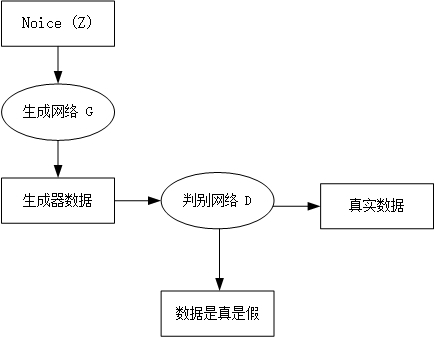
\includegraphics[width=0.5\linewidth]{screenshot001}
		\caption{GAN设计思路}
		\label{fig:screenshot001}
	\end{figure}
	GAN 包括两个模型,一个是生成模型 \(G\)(Generator),一个是判别模型 \(D\)(Discriminator)。它们的功能分别是:
	
	\(G\) 负责生成图片,接收一个随机的噪声 \(z\),通过该噪声生成图片,记为 \(G(z)\)。
	
	\(D\) 负责判别一张图片是否“真实”。其输入是 \(x\),代表一张图片,输出 \(D(x)\) 表示 \(x\) 为真实图片的概率。输出为 1 代表真实图片的概率为 100\%,而输出为 0 则代表图片不可能是真实的(真实实例来源于数据集,伪造实例来源于生成模型)。
	
	\textbf{有一个很好的比喻,就是枯叶蝶的演化过程类似于树叶,枯叶蝶不需要认识树叶,但能通过变异逃避捕食者(筛选器),这样的自然选择使枯叶蝶越来越像树叶。同理,生成器产生的图片概率分布也会越来越接近真实数据集的概率分布。}
	
\subsection{损失函数和训练策略}
\subsubsection{(1)损失函数:}
	\begin{align}
		\min_G \max_D V(D, G) = & \mathbb{E}_{x \sim p_{\text{data}}(x)} [\log D(x)] 
		& + \mathbb{E}_{z \sim p_z(z)} [\log (1 - D(G(z)))]
	\end{align}
	含义很直接,对生成器,尽可能让$\mathbb{E}_{z \sim p_z(z)} [\log (1 - D(G(z)))]$更小,也就是$D(G(z))$尽可能大,前半段不涉及z,当常数处理。\\
	对判别器,就是真图像判别的结果越接近1越好,假图像越接近0越好。

\subsubsection{训练策略:}
\begin{figure}[hb]
	\centering
	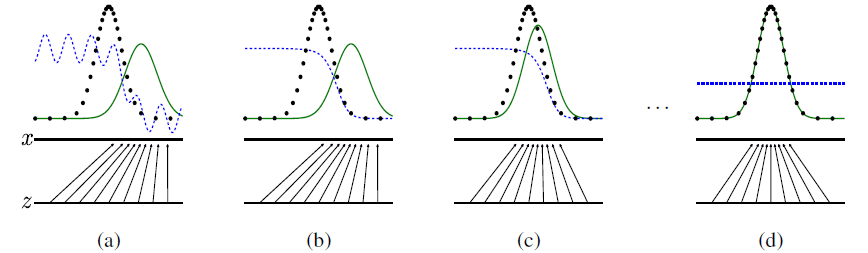
\includegraphics[width=0.7\linewidth]{screenshot002}
	\caption{(2)训练过程}
	\label{fig:screenshot002}
\end{figure}
\indent Note:判别器是小蓝,真实图片的概率分布是小黑,生成器整的映射是下半边的箭头,由全数据区域到生成的图像空间,绿色是生成图像空间的概率分布。
\begin{itemize}
	\item 生成器和真实图像的概率分布偏差大,性能是比较差,判别器虽然大体在真是图像概率大的地方高,但是不稳定。
	\item 判别器被迭代了几轮,区分良好。
	\item 生成器被迭代更新,概率分布趋近了真实图像分布一些。
	\item 重复上面两步...
	\item 大结局,以假乱真,判别器out。
\end{itemize}
\subsection{数学推导}
推荐文章:https://www.cnblogs.com/LXP-Never/p/9706790.html
\section{Code}
\href{run:GAN.ipynb}{点击这里查看代码文件:https://xiaolong-li1.github.io/Blogs/GAN/GAN.ipynb}
\subsubsection{(1):伪代码:}
\begin{algorithm}
	
	\begin{algorithmic}
		\label{alg:AGF}
		\FOR{number of training iterations}
		\FOR{$k$ steps}
		\STATE{$\bullet$ Sample minibatch of $m$ noise samples $\{ \bm{z}^{(1)}, \dots, \bm{z}^{(m)} \}$ from noise prior $p_g(\bm{z})$.}
		\STATE{$\bullet$ Sample minibatch of $m$ examples $\{ \bm{x}^{(1)}, \dots, \bm{x}^{(m)} \}$ from data generating distribution $p_\text{data}(\bm{x})$.}
		\STATE{$\bullet$ Update the discriminator by ascending its stochastic gradient:
			\[
			\nabla_{\theta_d} \frac{1}{m} \sum_{i=1}^m \left[
			\log D\left(\bm{x}^{(i)}\right)
			+ \log \left(1-D\left(G\left(\bm{z}^{(i)}\right)\right)\right)
			\right].
			\]}
		%parameters $\theta_d$ of discriminator $D$
		%in the direction of the stochastic gradient of the binomial cross-entropy
		%for $D$ predicting whether its argument comes from $p_\text{data}(\bm{x})$ (target = 1, input = $\bm{x}$) or
		%$P_g$ (target = 0, input = $G(\bm{z})$), i.e., towards minimizing
		% \mbox{$-\log D(\bm{x}) - \log(1 - D(G(\bm{z})))$}.}
	\ENDFOR
	\STATE{$\bullet$ Sample minibatch of $m$ noise samples $\{ \bm{z}^{(1)}, \dots, \bm{z}^{(m)} \}$ from noise prior $p_g(\bm{z})$.}
	\STATE{$\bullet$ Update the generator by descending its stochastic gradient:
		\[
		\nabla_{\theta_g} \frac{1}{m} \sum_{i=1}^m
		\log \left(1-D\left(G\left(\bm{z}^{(i)}\right)\right)\right)
		.
		\]}
	\ENDFOR
	\\The gradient-based updates can use any standard gradient-based learning rule. We used momentum in our experiments.
\end{algorithmic}
\end{algorithm}
\begin{figure}[htbp]
	\centering
	\begin{subfigure}[b]{0.4\linewidth}
		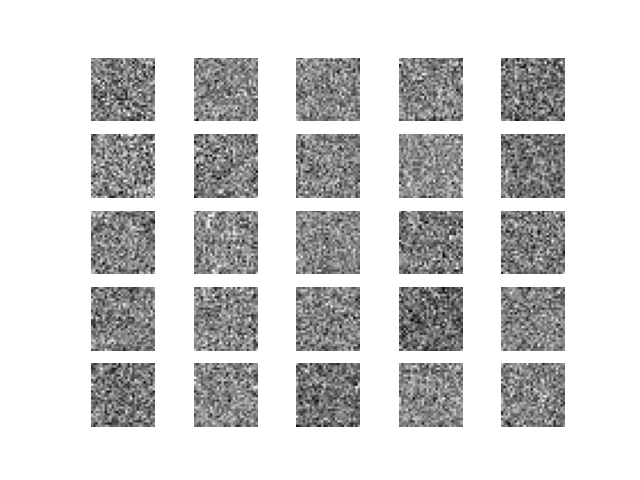
\includegraphics[width=\linewidth]{./images/0.png}
		\caption{训练0个epoch的生成结果}
		\label{fig:epoch0}
	\end{subfigure}
	\hfill % 添加一些水平空间
	\begin{subfigure}[b]{0.4\linewidth}
		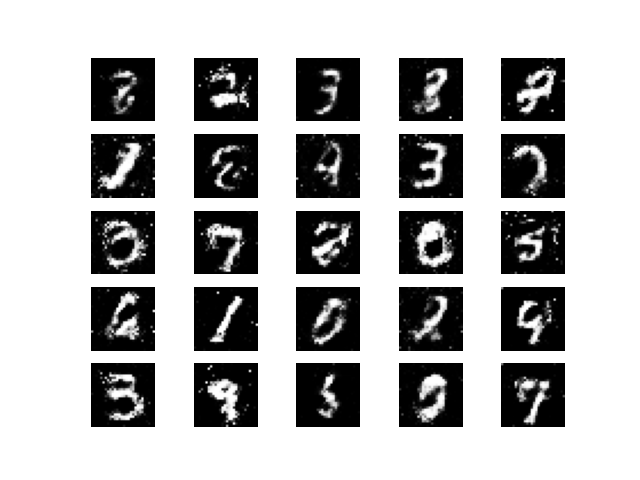
\includegraphics[width=\linewidth]{./images/200.png}
		\caption{训练200个epoch生成的结果}
		\label{fig:epoch200}
	\end{subfigure}
	\caption{训练不同epoch数的生成结果对比}
	\label{fig:epochs_comparison}
\end{figure}
\chapter{VAE model}
\section{设计思路}
\subsection{Auto Encoder结构}
\begin{figure}[h]
	\centering
	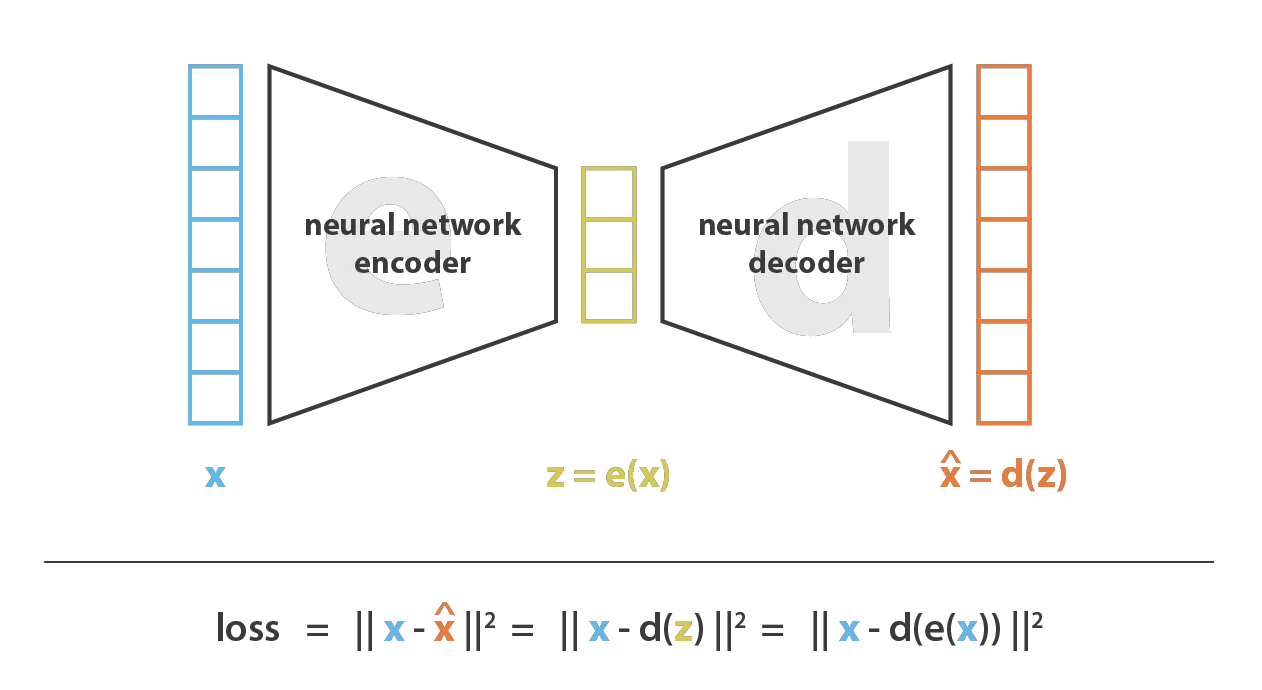
\includegraphics[width=0.7\linewidth]{images/screenshot006}
	\caption{Auto Encoder结构}
	\label{fig:screenshot006}
\end{figure}
\indent VAE结构基于AE,这种网络结构有一个很经典的功能,数据降维,可以把高维度的数据变成很低的维度,但是仍然保留大部分语义特征(因为它能通过一个固定的函数(解码器)以比较小的误差恢复出来)。至于这个网络能干什么,去噪,数据压缩之类的。
\begin{itemize}
	\item 这时候刚好来引入一个概念,\textbf{latent space}(我就叫它表示空间好了),也就是图中z向量所在的空间,
	\item 第二个概念是,latent space的正则性,这里用两幅图描述。
	\begin{figure}[t]
		\centering
		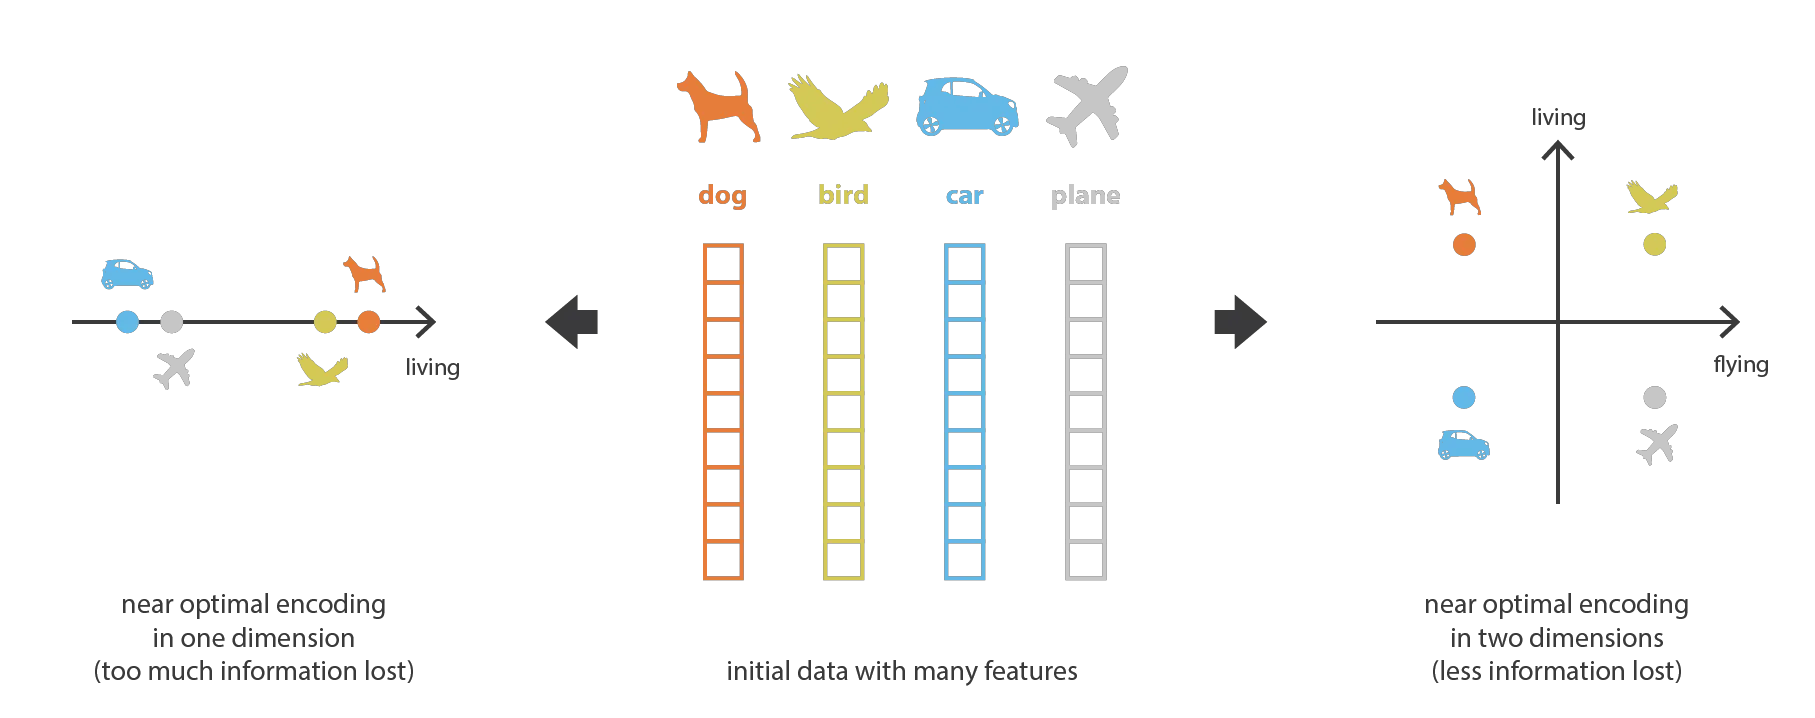
\includegraphics[width=1\linewidth]{images/screenshot007}
		\label{fig:screenshot007}
	\end{figure}
	\begin{figure}[h]
		\centering
		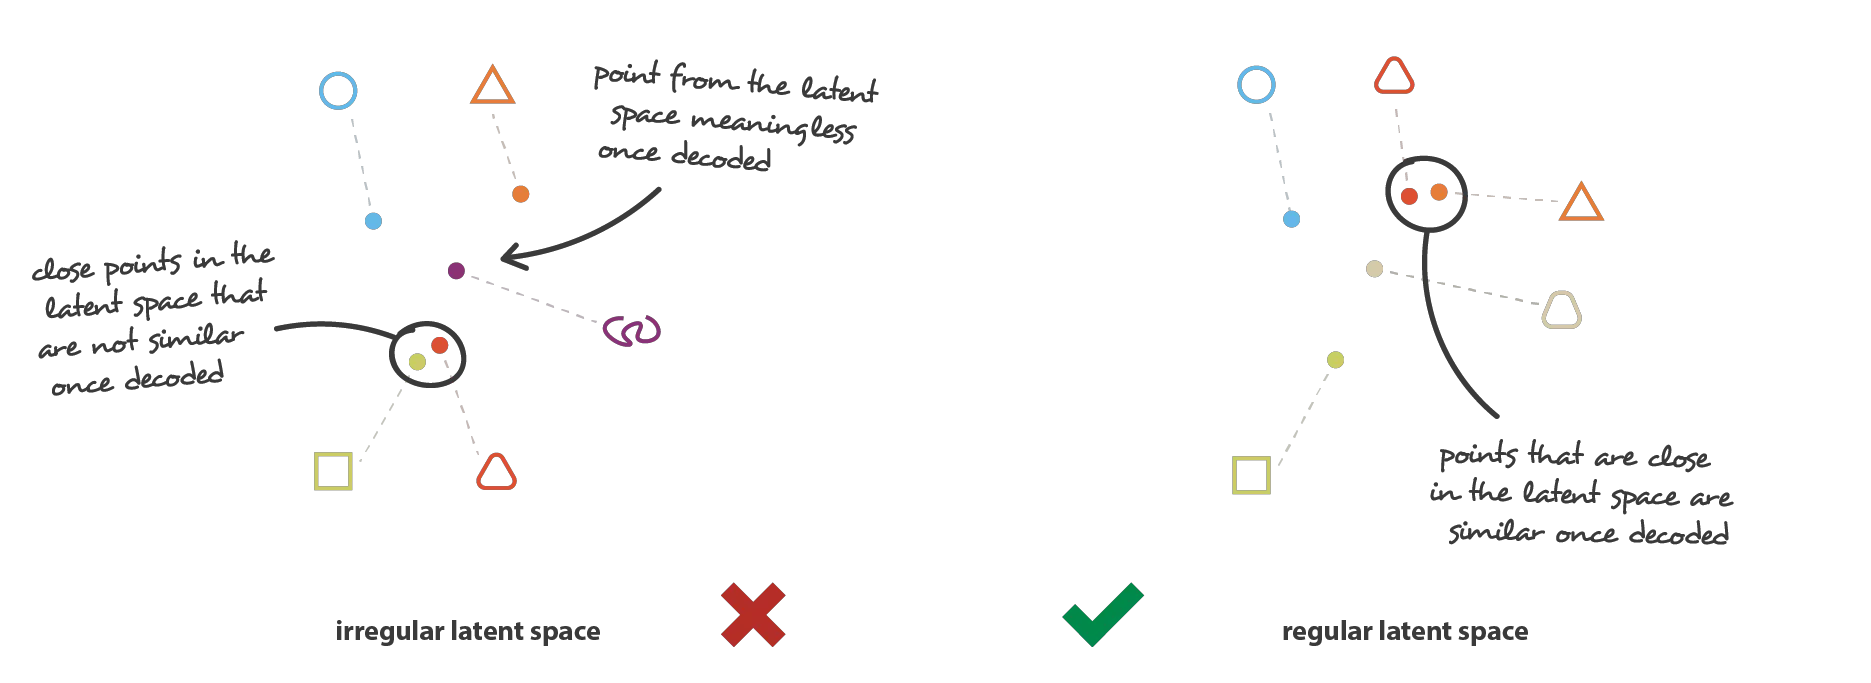
\includegraphics[width=1\linewidth]{images/screenshot008}
		\caption{正则化的直观感受}
		\label{fig:screenshot008}
	\end{figure}
	
	\FloatBarrier
	这里的左侧的表示空间和右侧比较就没什么结构,差别很大的东西在表示空间里的位置却没有散开,相似的没有聚在一堆。
\end{itemize}
\subsection{灵感乍现,这个decoder似乎有做图像生成的潜力}
\indent 它能用低维度的一些看似随机的向量整出来有意义的图片,如果我们直接随机生成一些向量输进去会不会也能搞出来新的作品?不过先考虑下面的要求。
\begin{enumerate}
	\item 随机的向量都能有图片对应,这说明一个事情,latent space的大部分空间都会在高维空间得有有意义的图像对应。我们原有的训练策略从没有对表示空间做任何要求,它可以就好多离得很远的片区有有意义的图像对应。
	\item 它一个输入绝对只有一个输出,这不好,我们应该生成多个类似的但又不一样的图像以供选择。
\end{enumerate}
\subsection{VAE怎么满足这些要求的?}
\subsubsection{VAE结构}
\begin{figure}[h]
	\centering
	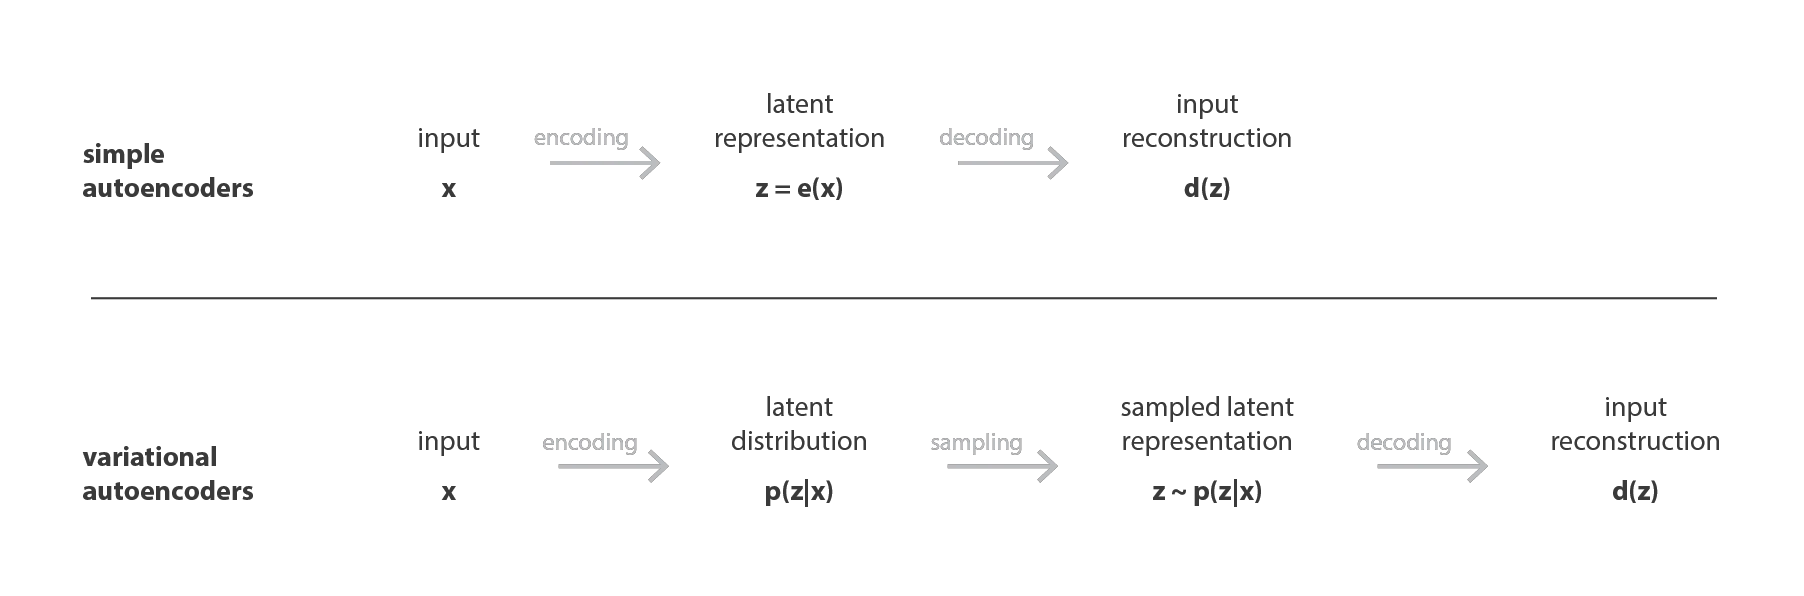
\includegraphics[width=0.8\linewidth]{images/screenshot012}
	\caption{VAE和AE区别}
	\label{fig:screenshot012}
\end{figure}
\FloatBarrier
它的编码器不再是和表征空间的一个点对应了,而是一个概率分布,解码器也是得到的一个概率分布,不过方差是提前固定的
\begin{figure}[ht]
	\centering
	\begin{subfigure}[b]{0.4\textwidth}
		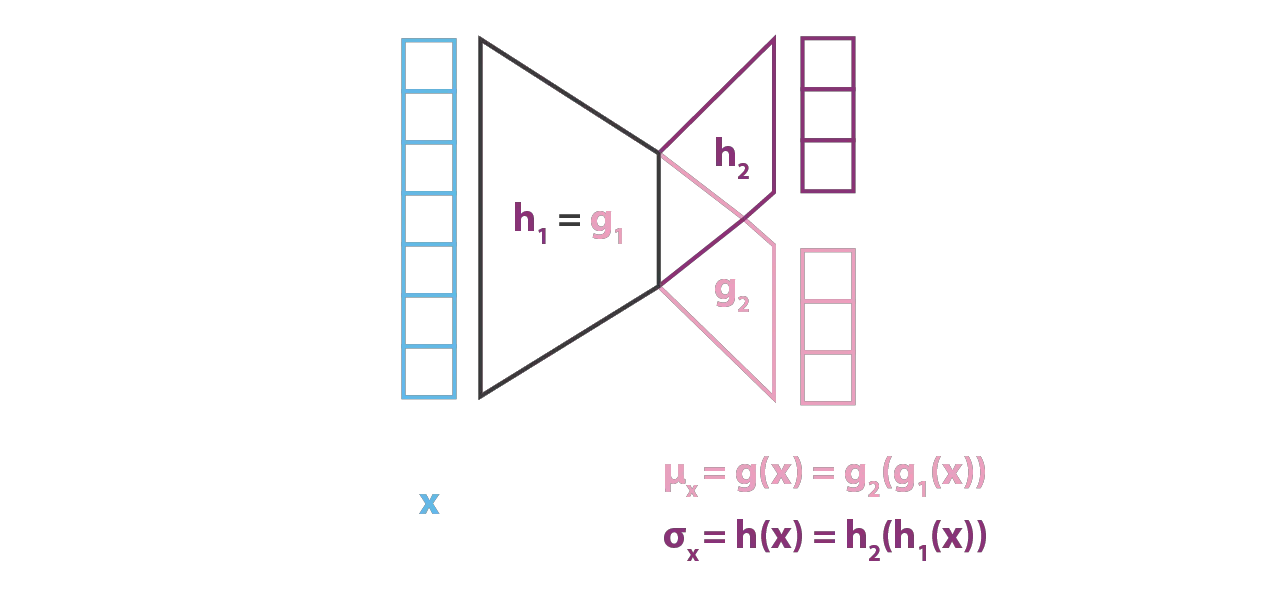
\includegraphics[width=\textwidth]{images/screenshot009}
		\caption{VAE编码器}
		\label{fig:screenshot009}
	\end{subfigure}
	\hfill % 添加一些水平空间或者使用 \quad, \qquad 等来调整子图之间的间距
	\begin{subfigure}[b]{0.4\textwidth}
		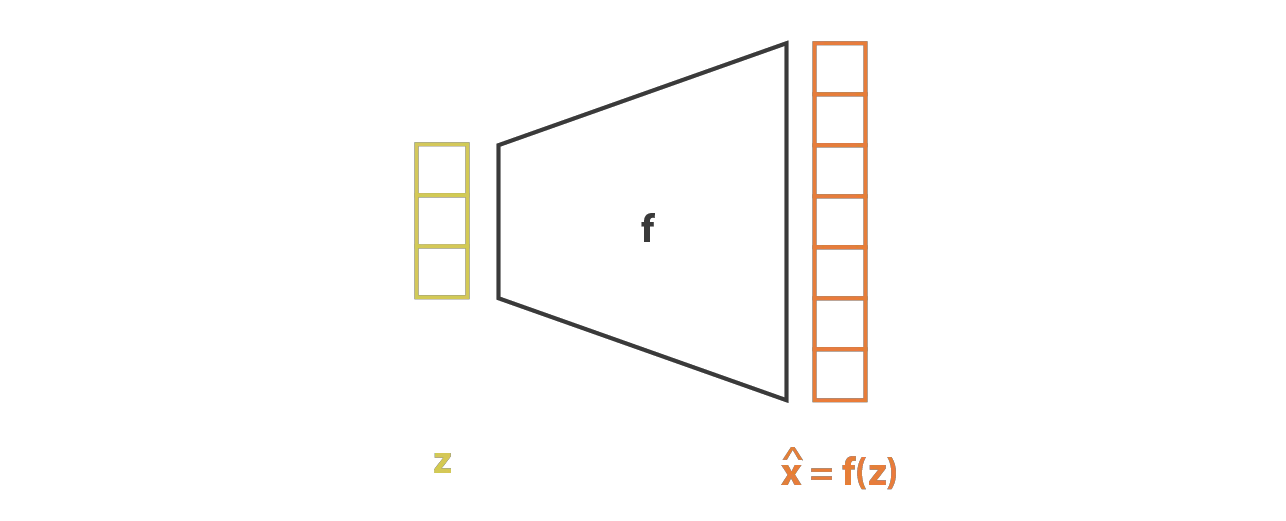
\includegraphics[width=\textwidth]{images/screenshot010}
		\caption{VAE解码器}
		\label{fig:sub2}
	\end{subfigure}
	\begin{subfigure}[b]{0.8\textwidth}
		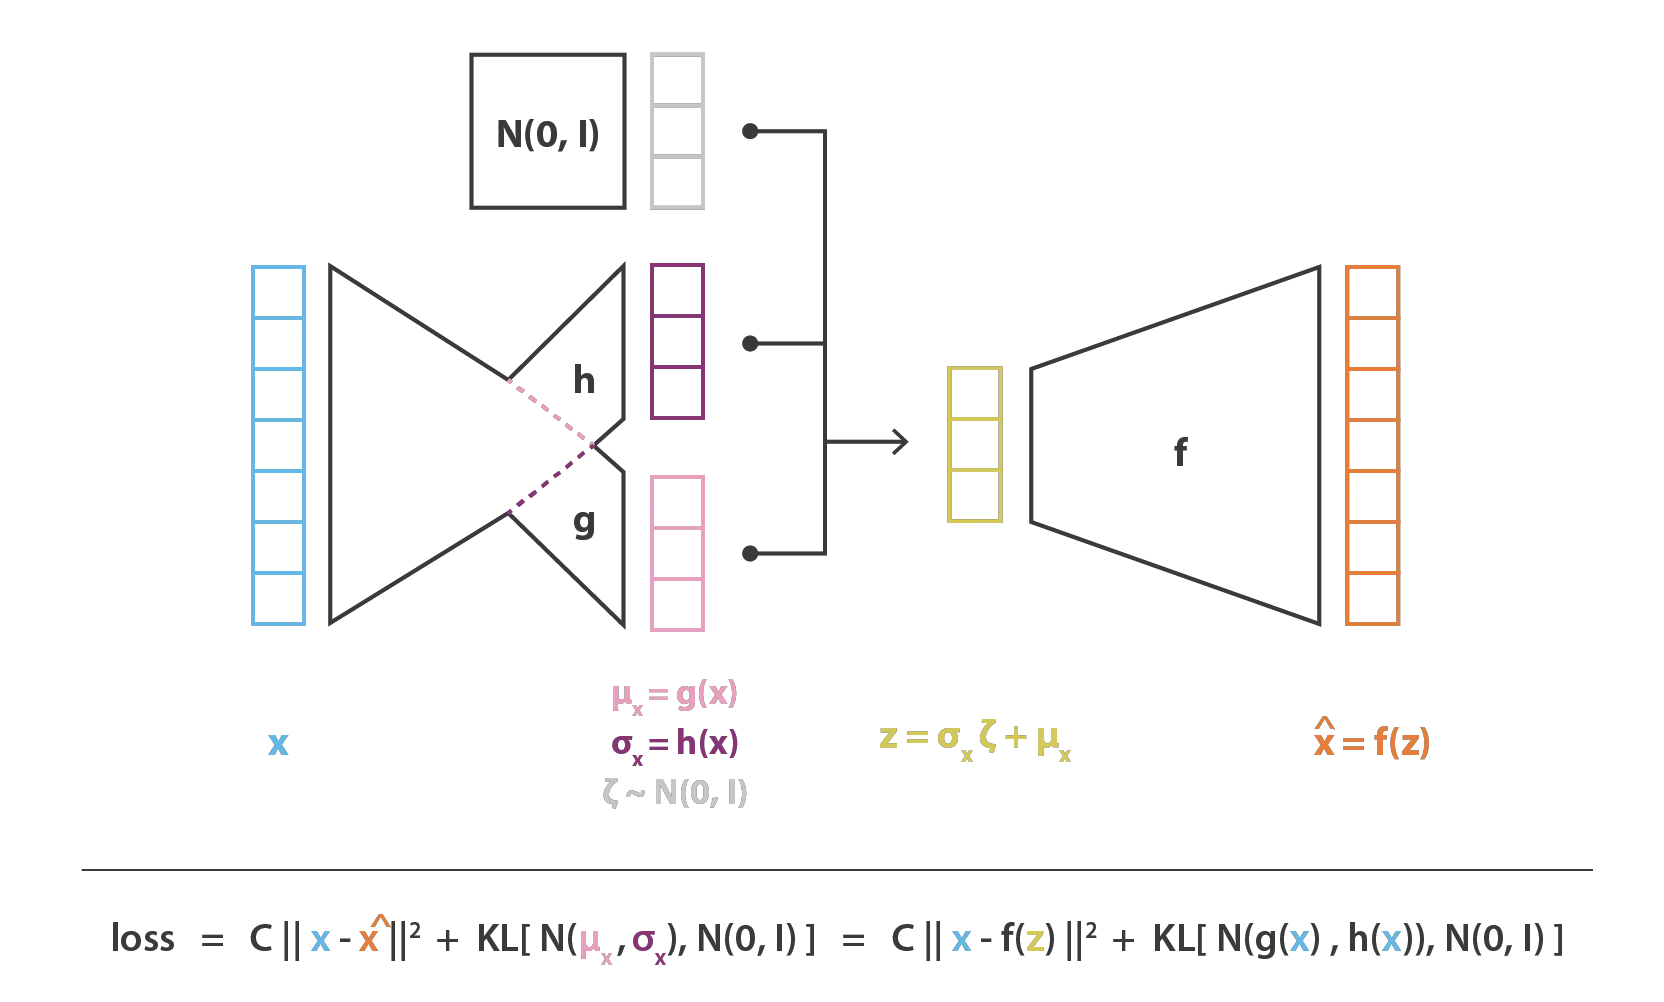
\includegraphics[width=\textwidth]{images/screenshot011}
		\caption{VAE整体结构}
		\label{fig:sub3}
		\end{subfigure}
	\caption{VAE结构}
	\label{fig:test}
\end{figure}
\FloatBarrier
\begin{itemize}
	\item 图a:解码器介绍:两部分构成的神经网络(前半边公用),输入是图像,输出是确定一种分布所需的参数(高斯分布为例,均值向量和协方差矩阵,不过为了减少计算量,假定各个特征也不相关,就成了方差向量了)
	\item 图b:编码器介绍:输入时从前面的分布从latent space采样的特征表示,输出是高斯分布的均值,实际上也就是输出图像的预期,有一个固定的方差,采样得到输出结果。
	\item 图c:整合的小策略:为了能让网络可以训练,特意用N(0,1)这个模块来帮助表示各种高斯分布,完成采样。
	\begin{figure}[h]
		\centering
		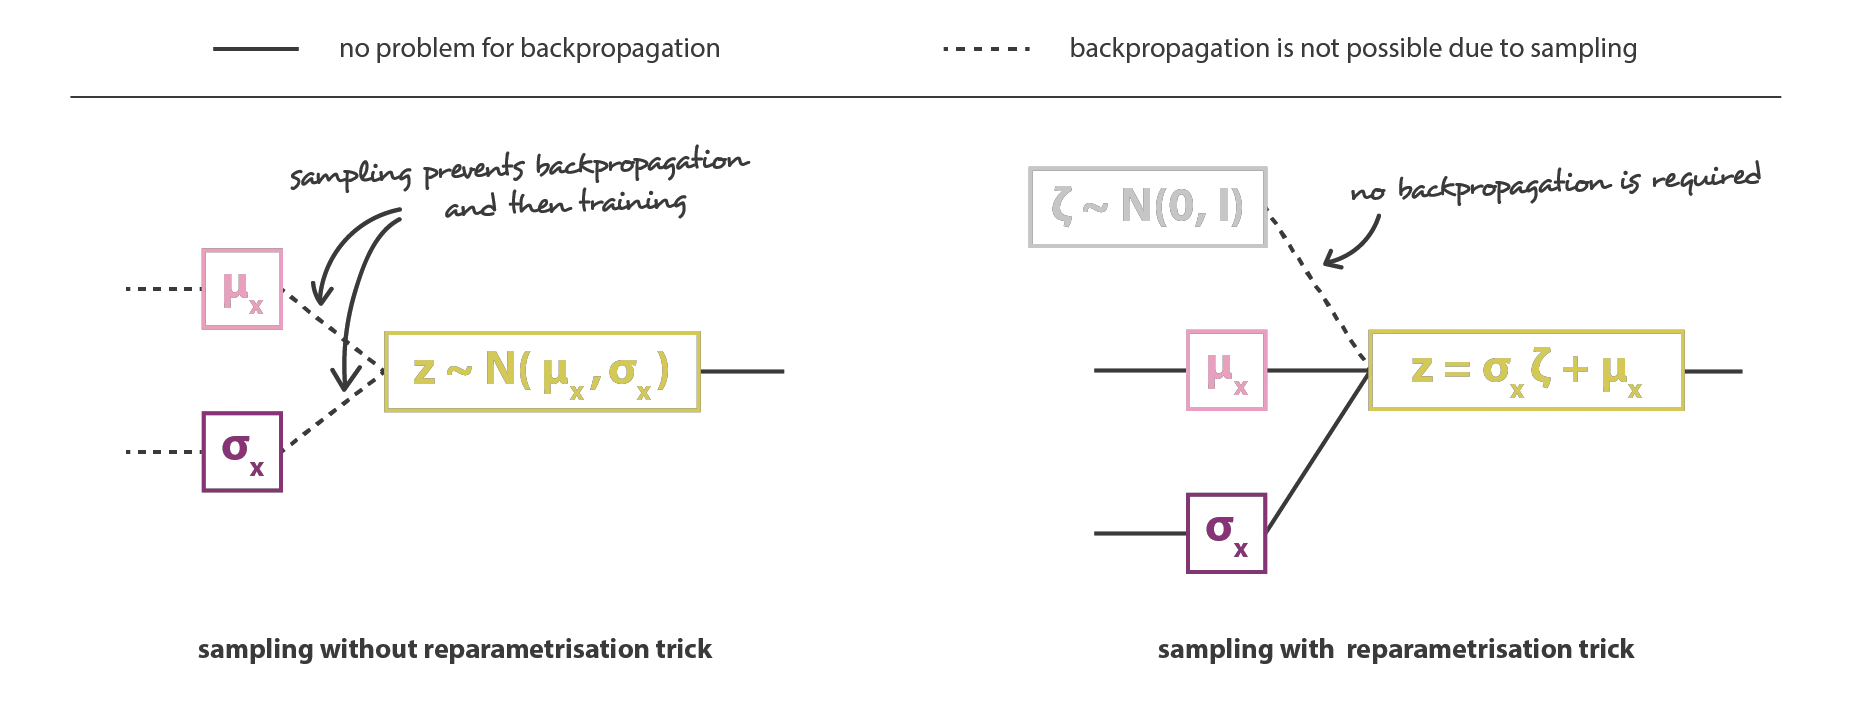
\includegraphics[width=0.7\linewidth]{images/screenshot013}
		\label{fig:screenshot013}
	\end{figure}
	
\end{itemize}
\subsubsection{进入正题}
VAE巧妙地用了概率分布作为编解码器映射的对象,而且选用高斯分布,训练时每一个真实样本,相当和表征空间的某个点为中心的一片区域对应上了,而且损失函数还要让这个概率分布接近$N(0,1)$,意味着映射的区域,或者点云都集中在一块,但又有一定的距离来确保准确性($\hat{x}-x$这个损失限制)

\section{损失函数怎么设计出来的?}
这里就进入了数学部分。\\
先定义
\begin{itemize}
	\item $x$:模型输入
	\item $z$:中间层的表示,在这个模型中是latent space采样后的结果
	\item $g(x)$: 输入:同编码器输入,输出:z所满足的高斯分布的均值
	\item $h(x)$: 输入:同编码器输入,输出:z所满足的高斯分布的方差
	\item $q_x(z)$ :  z的概率密度分布,$q_x(z) \equiv  \mathcal{N}(g(x),h(x)),g(x)\in G,h(x)\in  H;$\\ G H是函数族
\end{itemize}
再假设
\begin{itemize}
	\item $z$应该满足$\mathcal{N}$(0,1)
	\item $p(x|z)$也满足正态分布,方差是固定的,均值是通过解码器给出的。\,即$p(x|z)=\mathcal{N}(f(z),c)$
\end{itemize}
\newpage
$p(z|x)$根据上述假设,没法直接求出来,不过可以用正态分布函数族拟合,g和h是为了整出来一个正态分布来拟合$p(z|x)$
\begin{figure}[h]
	\centering
	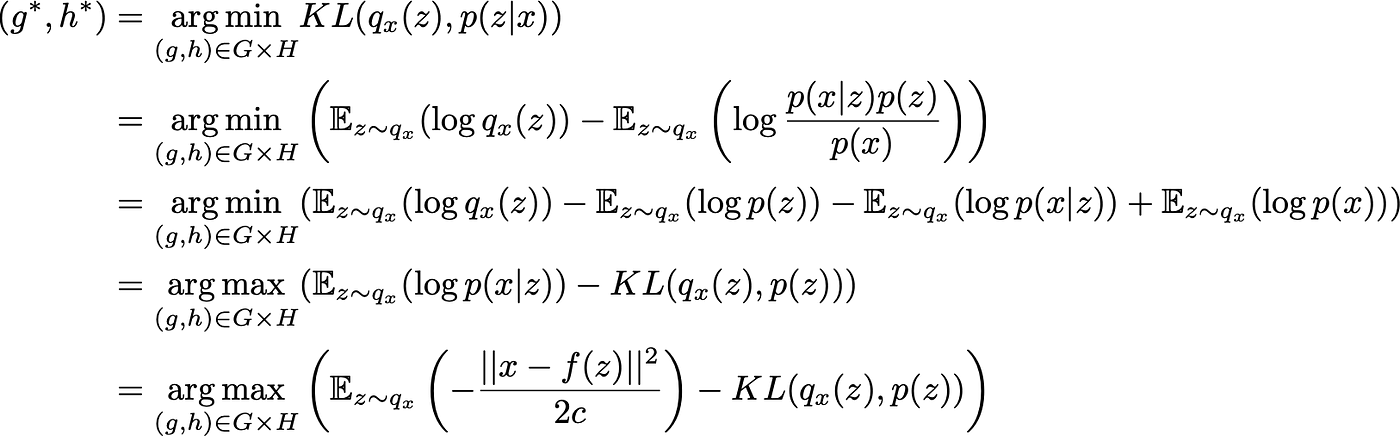
\includegraphics[width=0.9\linewidth]{images/screenshot014}
	\label{fig:screenshot014}
\end{figure}
\FloatBarrier
又因为解码器还要满足
\begin{figure}[h]
	\centering
	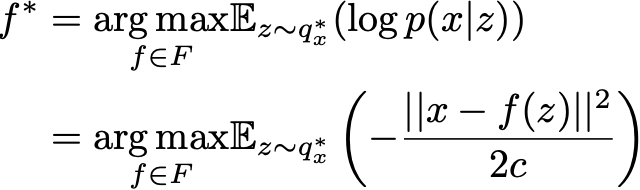
\includegraphics[width=0.4\linewidth]{images/screenshot015}
	\label{fig:screenshot015}
\end{figure}
就是得选一个好的解码器f能让$\hat{x}=x$的概率最高。\\
综合一下,就是要优化这个:\begin{figure}[h]
	\centering
	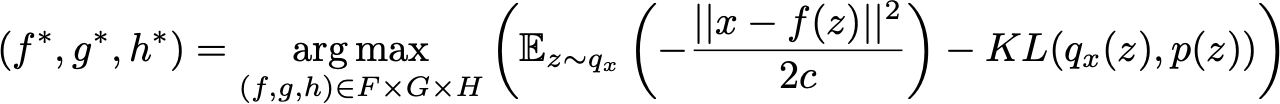
\includegraphics[width=0.8\linewidth]{images/screenshot016}
	\label{fig:screenshot016}
\end{figure}
\FloatBarrier
期望就在多轮的训练中间接实现,前后项可以加上一个权重,结合我们的假设,这就得到loss函数
\begin{align}
	Loss = \left\|x - \hat{x}\right\|^{2} + KL\left[\mathcal{N}(g(x), h(x)), \mathcal{N}(0, 1)\right]
\end{align}
另外,通过把KL散度的计算按照定义展开,再根据高斯分布的性质化简,可得:
\begin{align}
	KL(q(z|x) \parallel p(z)) = \frac{1}{2} \sum_{j=1}^{J} \left( \log(\sigma_j^2) + 1 - \sigma_j^2 - \mu_j^2 \right)
\end{align}
Note:\href{https://www.zywvvd.com/notes/study/probability/elbo/elbo/}{关于ELBO的文章:https://www.zywvvd.com/notes/study/probability/elbo/elbo/}
\section{Code:}
\href{./VAE.ipynb}{点击这里查看代码文件(https://xiaolong-li1.github.io/Blogs/GAN/VAE.ipynb)}
\chapter{Diffusion Model}
\section{简介}
\section{前向——加噪声}
在前向过程中,来自训练集的图像$x_0$会被添加T
次噪声,使得$x_T$
为符合标准正态分布。准确来说,「加噪声」并不是给上一时刻的图像加上噪声值,而是从一个均值与上一时刻图像相关的正态分布里采样出一幅新图像。如下面的公式所示,$\mathbf{x}_{T-1}$
是上一时刻的图像,$x_T$
是这一时刻生成的图像,该图像是从一个均值与
有关的正态分布里采样出来的。\\
\[
\mathbf{x}_t \sim \mathcal{N}(\mu_t(\mathbf{x}_{t-1}), \sigma_t^2 \mathbf{I})
\]
绝大多数扩散模型会把这个正态分布设置为这个形式:
\[
\mathbf{x}_t \sim \mathcal{N}(\sqrt{1-\beta_t}\mathbf{x_{t-1}},\beta_t \mathbf{I})
\]
\indent 这个正态分布公式乍看起来很奇怪:$\sqrt{1-\beta_t}$
是哪里冒出来的?为什么会有这种奇怪的系数?别急,我们先来看另一个问题:假如给定$\mathbf{x}_{0}$
,也就是从训练集里采样出一幅图片,该怎么计算任意一个时刻T
的噪声图像
呢?

我们不妨按照公式,从
开始倒推。
其实可以通过一个标准正态分布的样本
算出来:
\[
\begin{aligned}
	\mathbf{x}_t &\sim \mathcal{N}(\sqrt{1 - \beta_t}\mathbf{x}_{t-1}, \beta_t \mathbf{I}) \\
	&\Rightarrow \mathbf{x}_t = \sqrt{1 - \beta_t} \mathbf{x}_{t-1} + \sqrt{\beta_t} \epsilon_{t-1}; \epsilon_{t-1} \sim \mathcal{N}(0, \mathbf{I}) \\
	\\
	\mathbf{x}_t &= \sqrt{1 - \beta_t} \mathbf{x}_{t-1} + \sqrt{\beta_t} \epsilon_{t-1} \\
	&= \sqrt{1 - \beta_t}(\sqrt{1 - \beta_{t-1}}\mathbf{x}_{t-2} + \sqrt{\beta_{t-1}} \epsilon_{t-2}) + \sqrt{\beta_t} \epsilon_{t-1} \\
	&= \sqrt{(1 - \beta_t)(1 - \beta_{t-1})} \mathbf{x}_{t-2} + \sqrt{(1 - \beta_t)\beta_{t-1}} \epsilon_{t-2} + \sqrt{\beta_t} \epsilon_{t-1}
\end{aligned}
\]
由正态分布的性质可知,均值相同的正态分布「加」在一起后,方差也会加到一起。也就是\(\mathcal{N}(0, \sigma_1^2I)\)与\(\mathcal{N}(0, \sigma_2^2I)\)合起来会得到\(\mathcal{N}(0, (\sigma_1^2 + \sigma_2^2)I)\)。根据这一性质,上面的公式可以化简为:
\[
\begin{aligned}
&\sqrt{(1-\beta_t)(1-\beta_{t-1})}x_{t-2} + \sqrt{(1-\beta_t)\beta_{t-1}}\epsilon_{t-2} + \sqrt{\beta_t}\epsilon_{t-1}\\
&= \sqrt{(1-\beta_t)(1-\beta_{t-1})}x_{t-2} + \sqrt{(1-\beta_t)\beta_{t-1} + \beta_t}\epsilon\\
&= \sqrt{(1-\beta_t)(1-\beta_{t-1})}x_{t-2} + \sqrt{1-(1-\beta_t)(1-\beta_{t-1})}\epsilon
\end{aligned}
\]
再往前推一步的话,结果是:
\[
\sqrt{(1-\beta_t)(1-\beta_{t-1})(1-\beta_{t-2})}x_{t-3} + \sqrt{1-(1-\beta_t)(1-\beta_{t-1})(1-\beta_{t-2})}\epsilon
\]
我们已经能够猜出规律来了,可以一直把公式推到\(x_0\)。令\(\alpha_t = 1-\beta_t, \bar{\alpha}_t = \prod_{i=1}^t \alpha_i\),则:
\[
x_t = \sqrt{\bar{\alpha}_t}x_0 + \sqrt{1-\bar{\alpha}_t}\epsilon
\]
有了这个公式,我们就可以讨论加噪声公式为什么是\(x_t \sim \mathcal{N}(\sqrt{1-\beta_t}x_{t-1}, \beta_tI)\)了。这个公式里的\(\beta_t\)是一个小于1的常数。在DDPM论文中,\(\beta_t\)从\(\beta_1 = 10^{-4}\)到\(\beta_T = 0.02\)线性增长。这样,\(\beta_t\)变大,\(\alpha_t\)也越小,\(\bar{\alpha}_t\)超于0的速度越来越快。最后,\(\bar{\alpha}_T\)几乎为0,代入\(x_T = \sqrt{\bar{\alpha}_T}x_0 + \sqrt{1-\bar{\alpha}_T}\epsilon\),\(x_T\)就满足标准正态分布了,符合我们对扩散模型的要求。上述推断可以简单描述为:加噪声公式能够从慢到快地改变原图像,让图像最终均值为0,方差为I。

\section{反向——去噪声}
在正向过程中,我们人为设置了T
步加噪声过程。而在反向过程中,我们希望能够倒过来取消每一步加噪声操作,让一幅纯噪声图像变回数据集里的图像。这样,利用这个去噪声过程,我们就可以把任意一个从标准正态分布里采样出来的噪声图像变成一幅和训练数据长得差不多的图像,从而起到图像生成的目的。

现在问题来了:去噪声操作的数学形式是怎么样的?怎么让神经网络来学习它呢?数学原理表明,当$\beta_t$
足够小时,每一步加噪声的逆操作也满足正态分布。
\[
\mathbf{x}_{t-1} \sim \mathcal{N}\left(\tilde{\mu}_t, \tilde{\beta}_t \mathbf{I}\right)
\]
已知的:
\begin{align*}
	q\left(\mathbf{x}_{t-1} \mid \mathbf{x}_{t}, \mathbf{x}_0\right) &= q\left(\mathbf{x}_{t} \mid \mathbf{x}_{t-1}, \mathbf{x}_0\right) \frac{q\left(\mathbf{x}_{t-1} \mid \mathbf{x}_0\right)}{q\left(\mathbf{x}_{t} \mid \mathbf{x}_0\right)} \\
	q\left(\mathbf{x}_{t} \mid \mathbf{x}_0\right) &= \mathcal{N}\left(\mathbf{x}_{t}; \sqrt{\overline{\alpha}_t} \mathbf{x}_0, (1 - \overline{\alpha}_t) \mathbf{I}\right) \\
	q\left(\mathbf{x}_{t} \mid \mathbf{x}_{t-1}, \mathbf{x}_0\right) &= \mathcal{N}\left(\mathbf{x}_{t}; \sqrt{1 - \beta_t} \mathbf{x}_{t-1}, \beta_t \mathbf{I}\right)
\end{align*}
首先,把其他几个式子带入贝叶斯公式的等式右边。
\begin{align*}
	q(\mathbf{x}_{t-1}|\mathbf{x}_t,\mathbf{x}_0) &= \frac{1}{\beta_t \sqrt{2\pi}} \exp\left(-\frac{(\mathbf{x}_t - \sqrt{1 - \beta_t} \mathbf{x}_{t-1})^2}{2\beta_t}\right) \cdot \\
	&\quad \frac{1}{\left(1 - \overline{\alpha}_{t-1}\right)\sqrt{2\pi}} \exp\left(-\frac{\left(\mathbf{x}_{t-1} - \sqrt{\overline{\alpha}_{t-1}} \mathbf{x}_0\right)^2}{2\left(1 - \overline{\alpha}_{t-1}\right)}\right) \cdot \\
	&\quad \left(\frac{1}{\left(1 - \overline{\alpha}_t\right)\sqrt{2\pi}} \exp\left(-\frac{\left(\mathbf{x}_t - \sqrt{\overline{\alpha}_t} \mathbf{x}_0\right)^2}{2\left(1 - \overline{\alpha}_t\right)}\right)\right)^{-1}
\end{align*}
由于多个正态分布的乘积还是一个正态分布,我们知道$q\left( \mathbf{x}_{t-1} \mid \mathbf{x}_t, \mathbf{x}_0 \right)\sim \mathcal{N}(\tilde{\mu_t},\epsilon_t)$\\
\[
\epsilon_t=\tilde{\beta_t}
\]
\[
\tilde{\mu}_t = \frac{1}{\sqrt{\alpha_t}} \left( \mathbf{x}_t - \frac{1 - \alpha_t}{\sqrt{1 - \bar{\alpha}_t}} \epsilon_t \right)
\]
$\epsilon{t}$是用公式算$\mathbf{x}_t$
时从标准正态分布采样出的样本,它来自公式
\[
\mathbf{x}_t = \sqrt{\bar{\alpha}_t} \mathbf{x}_0 + \sqrt{1 - \bar{\alpha}_t} \epsilon_t
\]

\end{document}